\chapter{Podpunkt 1}
Sprawdzenie poprawności podanych wartości punktu pracy odbywa się poprzez zasymulowanie odpowiedzi procesu w punkcie pracy ($U_{\mathrm{pp}}$, $Y_{\mathrm{pp}}$). Z rys. \ref{Z1} widzimy, że podane wartości są poprawne.

\begin{figure}[ht]
\centering
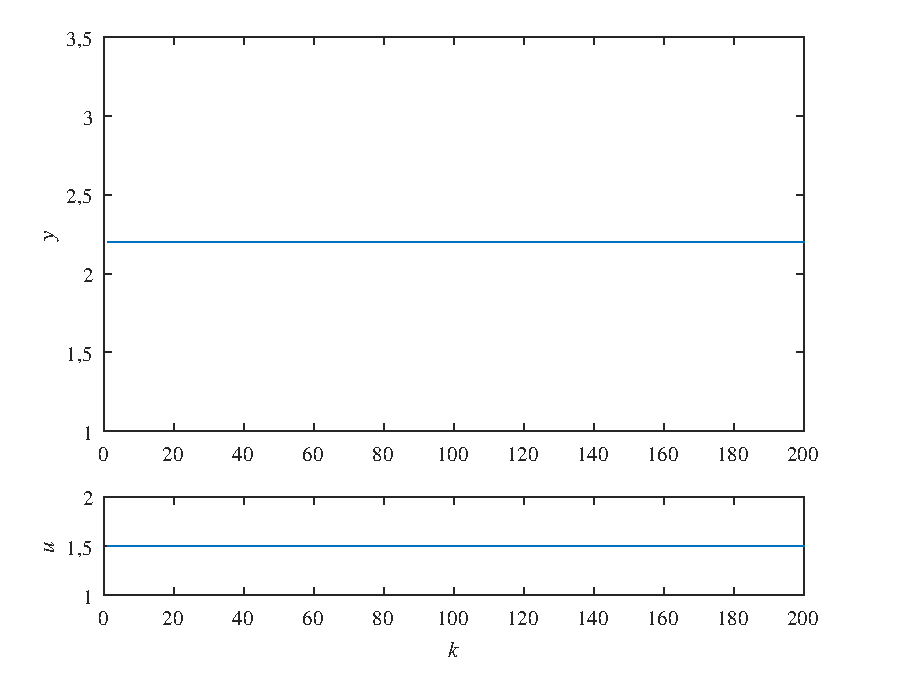
\includegraphics[scale=1]{images/Z1}
\caption{Odpowiedź procesu w punkcie pracy}
\label{Z1}
\end{figure}


\chapter{Podpunkt 2}
Po uwzględnieniu ograniczeń wartości sygnału sterującego dla reprezentacji odpowiedzi skokowych wybranych zostało sześć różnych wartości zmian sygnału sterującego. Wykres odpowiedzi skokowych zamieszczony został na rys. \ref{Z2multiplesteps}.

\begin{figure}[ht]
\centering
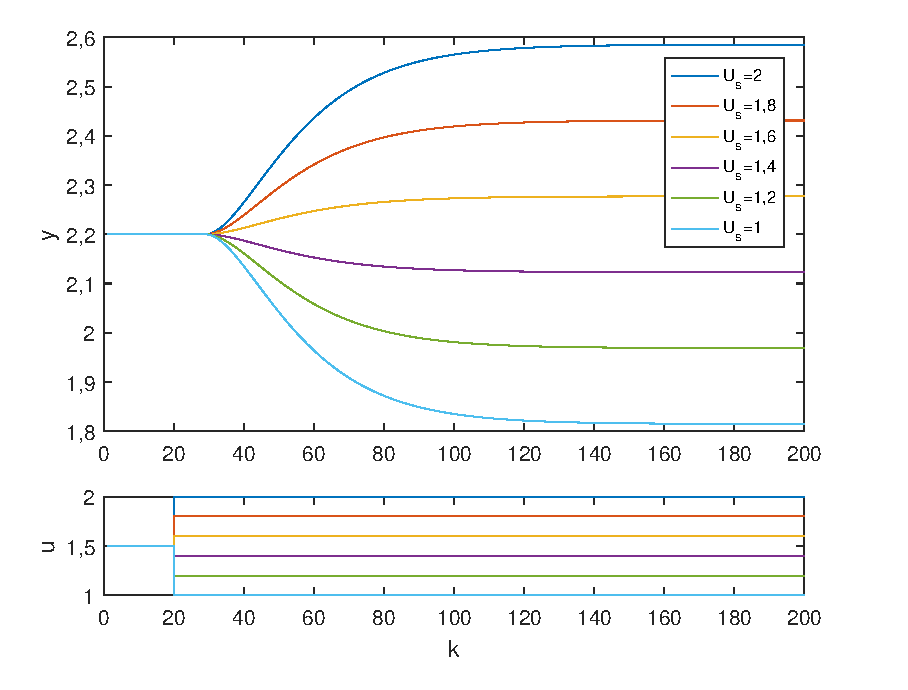
\includegraphics[scale=1]{images/Z2multiplesteps}
\caption{Wybrane odpowiedzi skokowe procesu}
\label{Z2multiplesteps}
\end{figure}

Symulując odpowiedź układu dla różnych wartości sygnału sterującego otrzymujemy charakterystykę statyczną $y(u)$ widoczną na rys. \ref{Z2staticchar}.


\begin{figure}[ht]
\centering
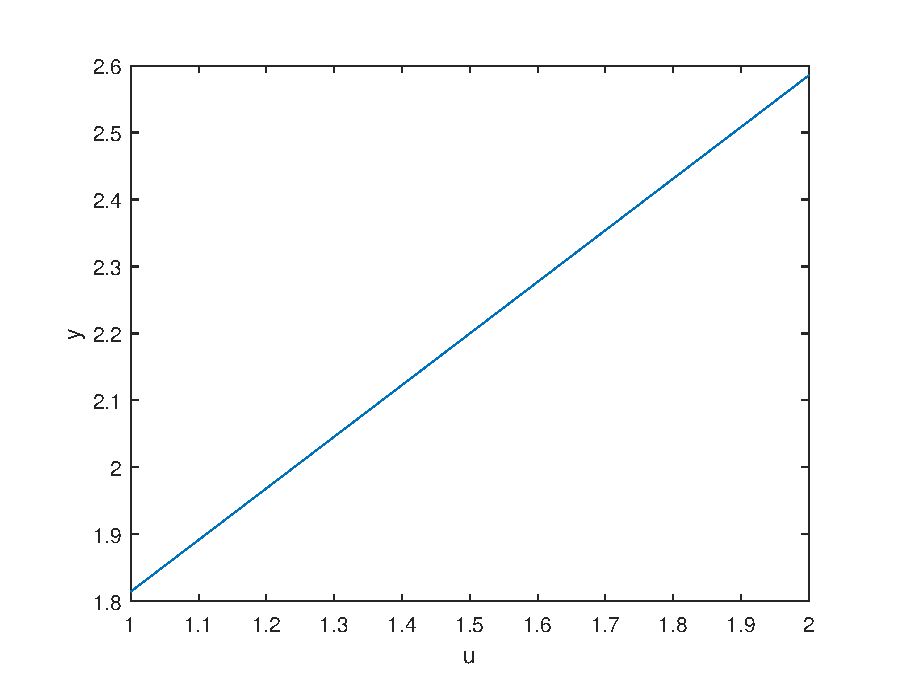
\includegraphics[scale=1]{images/Z2staticchar}
\caption{Charakterystyka statyczna procesu $y(u)$}
\label{Z2staticchar}
\end{figure}


Z odpowiedzi układu wnioskujemy, że właściwości statyczne i dynamiczne procesu są w bardzo dobrym przybliżeniu liniowe. Obliczona wartość wzmocnienia statycznego procesu to $K=\num{0,7706}$.


\chapter{Podpunkt 3}
Na potrzeby algorytmu DMC przekształcona została odpowiedź skokowa dla skoku z punktu pracy o wartość dopuszczoną przez ograniczenia, t.j. dla skoku od $U_{\mathrm{pp}}=\num{1,5}$ do $U^{\mathrm{max}}=\num{2,0}$. Do przekształcenia wykorzystany został wzór (\ref{step_norm}), zaś uzyskana odpowiedź skokowa została przedstawiona na rys. \ref{Z3step}.

\begin{equation}
S_i = \frac{S_i^0 - Y_{\mathrm{pp}}}{\triangle U} \textrm{, dla } i=1,\ldots
\label{step_norm}
\end{equation}


\begin{figure}[ht]
\centering
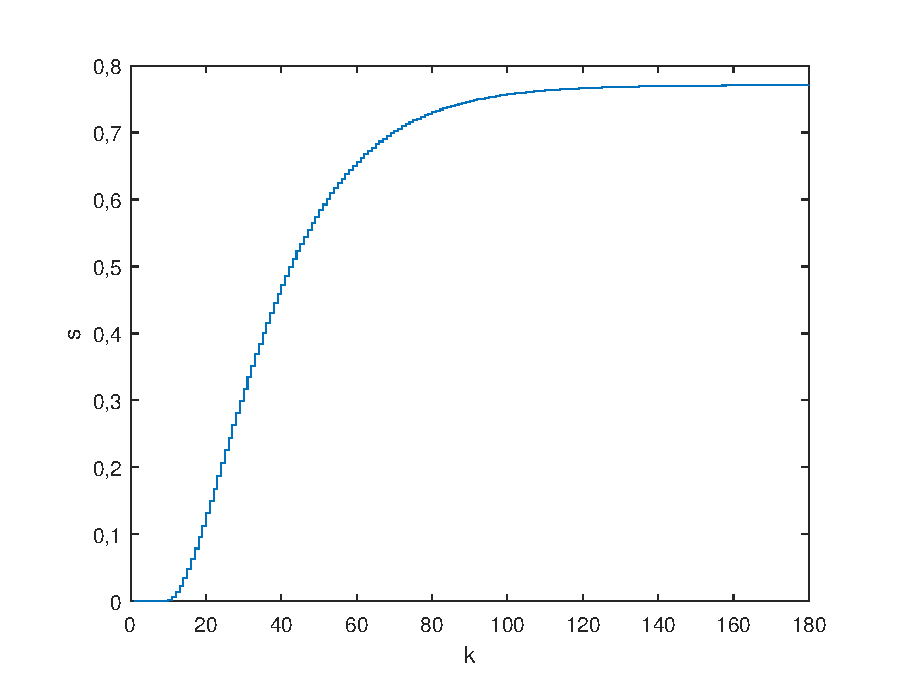
\includegraphics[scale=1]{images/Z3step}
\caption{Charakterystyka statyczna procesu $y(u)$}
\label{Z3step}
\end{figure}


\chapter{Podpunkt 4}
Programy do symulacji cyfrowej algorytmów PID oraz DMC (w wersji analitycznej) dla symulowanego procesu umieszczone zostały odpowiednio w plikach \verb+PID.m+, \verb+DMC.m+, zaś w plikach \verb+PID_err.m+ oraz \verb+DMC_err.m+ umieszczono funkcje pomocnicze do obliczania wartości błędu.


\chapter{Podpunkt 5}
Jakość regulacji oceniania była jakościowo na podstawie przebiegów oraz ilościowo zgodnie z zadanym wskaźnikiem jakości regulacji

\begin{equation}
E = \sum_{k=1}^{k_{\mathrm{konc}}}(y^{\mathrm{zad}}(k) - y(k))^2
\label{E}
\end{equation}

gdzie za koniec symulacji przyjęto $k_{\mathrm{konc}}=3000$. Dla

\begin{figure}[ht]
\centering
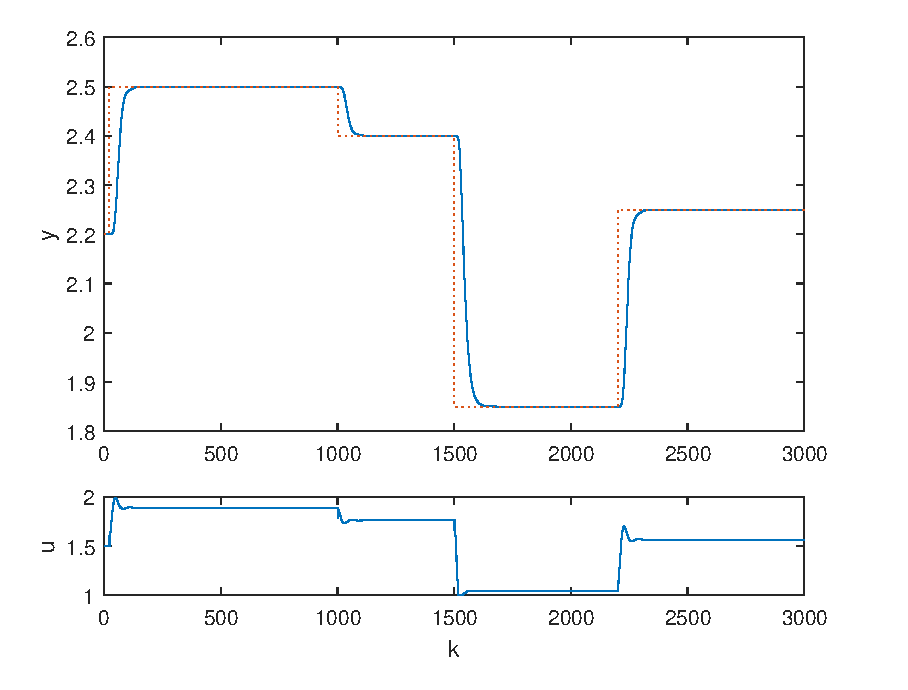
\includegraphics[scale=1]{images/Z5manualPID}
\caption{Wyniki symulacji dla dobranego eksperymentalnie regulatora PID, $E=\num{0}$}
\label{Z5manualPID}
\end{figure}


\begin{figure}[ht]
\centering
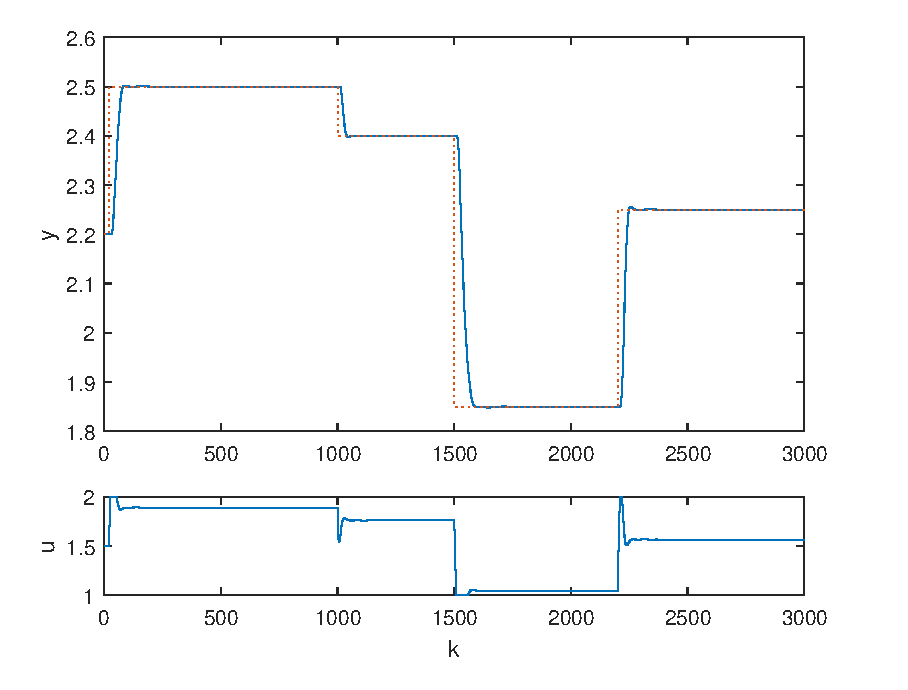
\includegraphics[scale=1]{images/Z5manualDMC}
\caption{Wyniki symulacji dla dobranego eksperymentalnie regulatora DMC, $E=\num{0}$}
\label{Z5manualDMC}
\end{figure}

\chapter{Podpunkt 6}


\begin{figure}[ht]
\centering
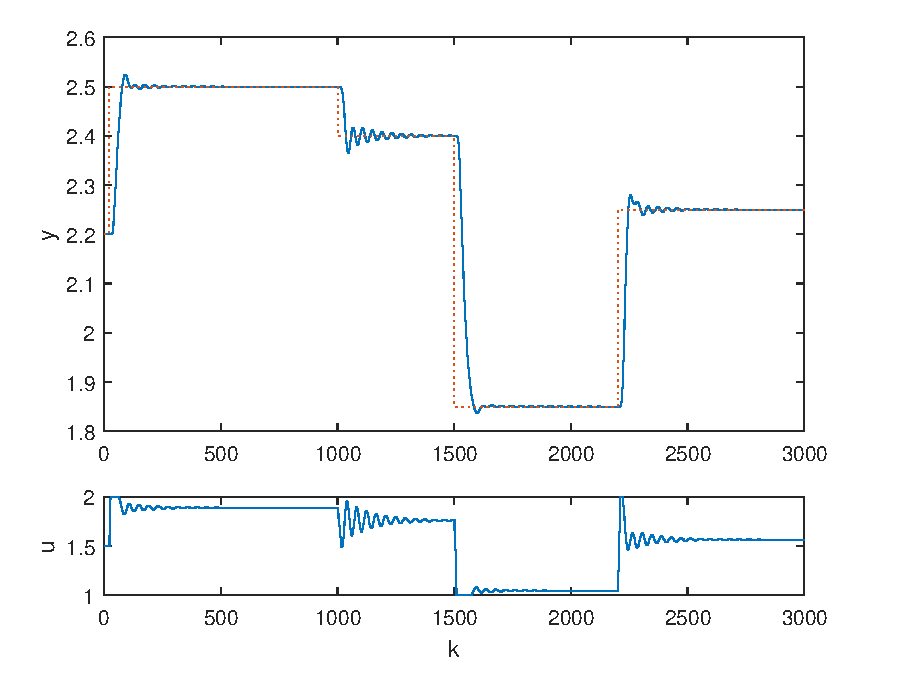
\includegraphics[scale=1]{images/Z6optimizedPID}
\caption{Wyniki symulacji dla regulatora PID otrzymanego w wyniku optymalizacji, $E=\num{0}$}
\label{Z6optimizedPID}
\end{figure}


\begin{figure}[ht]
\centering
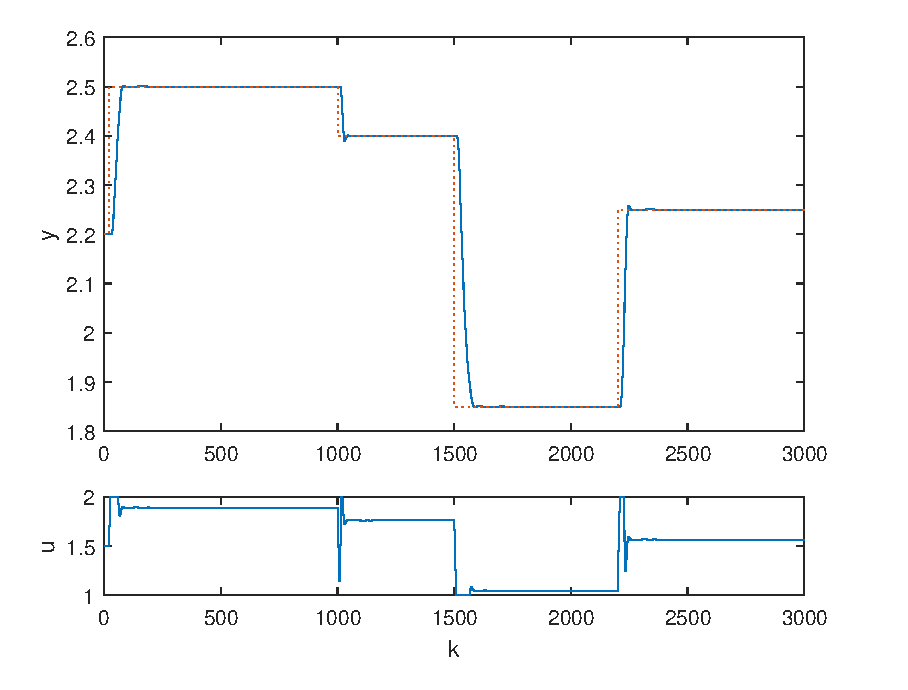
\includegraphics[scale=1]{images/Z6optimizedDMC}
\caption{Wyniki symulacji dla regulatora DMC otrzymanego w wyniku optymalizacji, $E=\num{0}$}
\label{Z6optimizedDMC}
\end{figure}
